%==============================================================
%  Disk Guard AI Agent — IEEE conference manuscript (IEEEtran)
%  Compile:   pdflatex disk-guard && bibtex disk-guard && pdflatex disk-guard && pdflatex disk-guard
%  Or:        make           (see Makefile)
%  Or:        upload to Overleaf and click Recompile
%==============================================================

\documentclass[conference]{IEEEtran}
\IEEEoverridecommandlockouts

\usepackage{cite}
\usepackage{amsmath,amssymb,amsfonts}
\usepackage{algorithmic}
\usepackage{graphicx}
\usepackage{textcomp}
\usepackage{xcolor}
\usepackage{booktabs}
\usepackage{array}
\usepackage{url}
\usepackage[hidelinks]{hyperref}
\usepackage{listings}

\graphicspath{{figures/}}

\lstset{
  basicstyle=\ttfamily\footnotesize,
  breaklines=true,
  frame=single,
  numbers=none,
  showstringspaces=false,
}

\begin{document}

\title{Disk Guard AI Agent: A Predictive Multi-AI Architecture for
Proactive Disk-Failure Prevention in Production Server Fleets}

\author{
\IEEEauthorblockN{Naga Raju Pitchuka}
\IEEEauthorblockA{
Tata Consultancy Services\\
Email: \href{mailto:rajupitchuka@gmail.com}{rajupitchuka@gmail.com}\\
GitHub: \url{https://github.com/rajupitchuka/disk-guard-AIagent}
}
}

\maketitle

%==============================================================
\begin{abstract}
Disk-fill incidents are among the most common production failures in
enterprise IT. From years supporting infrastructure operations at TCS,
I have watched the same pattern play out hundreds of times: a disk
fills up, a monitoring tool fires an alert at 85--90\% utilization, a
ticket lands in the queue, and an on-call engineer logs in to clean
up before the volume saturates. Sometimes the engineer wins this
race. For anomalous fast-fill scenarios---runaway loggers, retry
storms, deploy regressions---the alert fires too late and the host
goes down. The economic cost is significant: industry surveys put
enterprise hourly outage cost above USD 300K
\cite{itic2022downtime,lerner2014downtime}, and storage-related events
account for roughly 10--15\% of infrastructure incidents
\cite{notaro2021aiops}. At the scale of a typical 3{,}000-server
estate, disk-fill alone consumes on the order of one engineering FTE
per year and produces several million dollars per year in associated
outage cost; the global aggregate runs into the tens of billions of
US dollars annually. This paper describes \textbf{Disk Guard AI
Agent}, a working proof of concept that addresses this structurally.
Rather than waiting for thresholds, the system continuously forecasts
disk saturation using Prophet \cite{taylor2018forecasting} and
classifies anomalous growth using XGBoost \cite{chen2016xgboost}.
When either signal crosses a trigger condition, a Claude-powered
LangGraph agent \cite{anthropic2024claude3,langchain2024langgraph}
grounded in retrieved past-incident records \cite{lewis2020rag}
reasons about the situation and produces a structured recommendation
(clean / escalate / wait). A Decision Engine then routes the
recommendation to one of three governance bands---auto-remediate,
chatbot approval, or ServiceNow ticket only---based on a confidence
score combining LLM self-confidence, ML signal alignment, RAG
grounding, and environment risk. The implementation is end-to-end on
a 53-host fleet with full ML cycles in approximately 8 seconds. Two
reproducible scenarios---a 16~GB predictive cleanup, and a
correctly-refused cleanup of an anomalous-growth event with an
auto-filed P2 ticket---demonstrate the system. The contribution is
not a new ML algorithm but a working composition pattern that
generalizes to other infrastructure-operations problems.
\end{abstract}

\begin{IEEEkeywords}
AIOps, predictive monitoring, agentic AI, retrieval-augmented
generation, time-series forecasting, anomaly detection, IT operations,
governance AI, large language models, site reliability engineering.
\end{IEEEkeywords}

%==============================================================
\section{Introduction}

Storage exhaustion is one of the more boring categories of production
failure. It is also one of the most common. In the years I have spent
supporting infrastructure operations for enterprise customers,
disk-fill incidents have been a constant background hum in the
on-call rotation. The broader discipline of preventing operational
failure has been formalized in the Site Reliability Engineering
literature \cite{beyer2016sre}, and a fairly active research community
has applied machine learning to the problem of failure prediction in
cloud and enterprise systems \cite{notaro2021aiops,salfner2010survey,
lin2018predicting}. Despite this, the dominant practical approach in
industry remains threshold-based reactive monitoring---and disk-fill
incidents keep happening.

The pattern repeats almost without variation. A host's monitored
partition (typically \texttt{/var/log} on a Linux web or app server,
or \texttt{C:\textbackslash Logs} on a Windows IIS server) fills
steadily over hours or days. Free space crosses a configured
threshold, most often 85\% or 90\% utilization, and the monitoring
agent emits an event. The event lands in a centralized observability
platform, an incident ticket is opened, and someone---either an
on-call engineer or, in better-instrumented teams, an automated
runbook---is dispatched to investigate.

This is reactive by design. Action only begins after a threshold
breach. The threshold has to be conservative or the team drowns in
false alarms. The response cycle includes human or automation
latency. For routine log accumulation it works well enough. For the
anomalous cases---a misconfigured logger left enabled in production,
an unbounded retry loop, an exception storm triggered by a bad
deploy---it does not. In those cases the disk does not fill
gradually. It fills in minutes, leaps over the threshold rather than
crossing it slowly, and saturates before any responder can react.
The result is a production outage that everyone agrees, after the
fact, was preventable.

This paper introduces \textbf{Disk Guard AI Agent}: a predictive,
multi-AI-component system that monitors continuously, forecasts the
trajectory in real time, reasons about whether observed growth is
normal or anomalous, and acts under explicit governance guardrails
\emph{before} the disk reaches a state requiring emergency
intervention. The system is implemented end-to-end as a working
proof of concept and validated on a fleet of 53 hosts. The full
source code, architecture diagrams, and reproduction scripts are
publicly available at the repository cited above. I built this
because I have lived the problem; the paper is a deliberate attempt
to share the solution pattern in a form other practitioners can pick
up, run, and adapt.

\subsection{Contributions}
\begin{enumerate}
\item A complete reference architecture for predictive disk
management, organized into four well-defined zones (Data, AI Agent,
Governance, Infrastructure) that map cleanly onto existing enterprise
tooling.
\item An implementation pattern combining time-series forecasting
\cite{taylor2018forecasting}, anomaly classification
\cite{chen2016xgboost}, retrieval-augmented LLM reasoning
\cite{lewis2020rag}, and confidence-scored governance into a coherent
decision pipeline.
\item A demonstration of how a state-of-the-art language model, when
grounded in retrieved runbook + past-incident content, makes
operationally sensible distinctions---most notably refusing to clean
files when growth is anomalous and would mask an upstream incident,
and instead escalating via ServiceNow.
\item An open-source POC, including a Streamlit demonstration UI
structured around the operator workflow Monitor $\rightarrow$
Predict $\rightarrow$ Reason $\rightarrow$ Resolve, that allows the
system's behavior to be observed, validated, and reproduced.
\end{enumerate}

\subsection{Paper Organization}
Section \ref{sec:problem} reviews the limits of traditional reactive
monitoring and the economic scale of the problem. Section
\ref{sec:approach} introduces the predictive paradigm and contrasts
the two approaches against a common incident scenario. Section
\ref{sec:architecture} presents the reference architecture. Section
\ref{sec:impl} details the implementation. Section \ref{sec:flow}
walks through the operational workflow. Section \ref{sec:validation}
describes validation. Section \ref{sec:discussion} discusses
limitations and production considerations. Section \ref{sec:future}
outlines future work. Section \ref{sec:conclusion} concludes.

%==============================================================
\section{The Problem: Limits of Reactive Disk Monitoring}
\label{sec:problem}

\subsection{Scope and Economic Impact}

Before describing the operational model, it is worth establishing
how big the disk-fill problem actually is in financial and human
terms. Quantifying this precisely is hard because enterprises rarely
publish per-incident-class outage data, but several reference points
support a defensible estimate.

\textbf{Per-hour outage cost.} The widely-cited Gartner figure of
USD 5{,}600 per minute (approximately USD 336K per hour) of IT
downtime \cite{lerner2014downtime} remains a reasonable mean across
the enterprise survey base. ITIC's annual \emph{Hourly Cost of
Downtime} surveys consistently report that the majority of
enterprises peg an hour of unplanned downtime above USD 300K, with
the top tier (financial services, telecommunications, healthcare)
frequently citing figures above USD 1M per hour for customer-facing
systems \cite{itic2022downtime}.

\textbf{Incident-category share.} Storage and disk-related events
typically account for 10--15\% of infrastructure incidents in
mid-to-large estates \cite{notaro2021aiops,salfner2010survey}.

\textbf{Manual effort per incident.} A typical disk-related ticket
consumes 45--90 minutes of L2/L3 engineering time. At a fully-loaded
enterprise SRE rate of USD 80--120 per hour, this is roughly USD
80--150 per ticket in labor cost alone.

Applying these reference points across enterprise size segments
produces the rough estimates summarized in Table~\ref{tab:market}.

\begin{table*}[t]
\centering
\caption{Estimated annual cost of disk-fill incidents by enterprise
segment. Numbers assume an industry-typical 1--2\% annual
disk-incident rate per server, with 10--25\% of incidents escalating
to customer-facing outage. Outage cost per event is conservative
relative to Gartner / ITIC means.}
\label{tab:market}
\begin{tabular}{lrrrrr}
\toprule
\textbf{Segment} & \textbf{Servers} & \textbf{Disk inc./yr} &
\textbf{Eng.\ effort} & \textbf{Outage cost/yr} &
\textbf{Total burden} \\
\midrule
Small (1--50 servers, USD 10--50M rev.)        & \textasciitilde 25    & 5--15        & 10--25 hr           & USD 5--15K   & USD 10--25K \\
Medium (50--500 servers, USD 50M--1B rev.)     & \textasciitilde 250   & 50--150      & 75--225 hr          & USD 250--500K & USD 300--550K \\
Large (500--10{,}000+ servers, USD 1B+ rev.)   & \textasciitilde 3{,}000 & 1{,}000--3{,}000 & 1{,}500--4{,}500 hr ($\approx$ 1--2 FTE) & USD 7--15M    & USD 7--15M \\
\bottomrule
\end{tabular}
\end{table*}

For a Fortune-500 IT estate with 5{,}000 production servers, an
industry-typical 1.5\% annual incident rate, and a 20\% subset
escalating to customer-facing outages, the model produces
approximately 75 outage-impacting events per year. At a conservative
USD 200K average outage cost (well below the Gartner mean), this is
approximately USD 15M per year in direct outage cost, plus USD
300--500K per year in unproductive engineering effort.

\textbf{Aggregate scale.} Taking the global population of enterprises
operating 500+ server estates as roughly 30{,}000 organizations, and
applying even the low end of the Large-segment burden range, the
collective annual cost of disk-fill incidents alone is in the
\textbf{tens of billions of US dollars} range. This is not a niche
problem.

\subsection{The Current Operational Model}

Figure \ref{fig:traditional} illustrates the prevailing pattern.

\begin{figure*}[t]
\centering
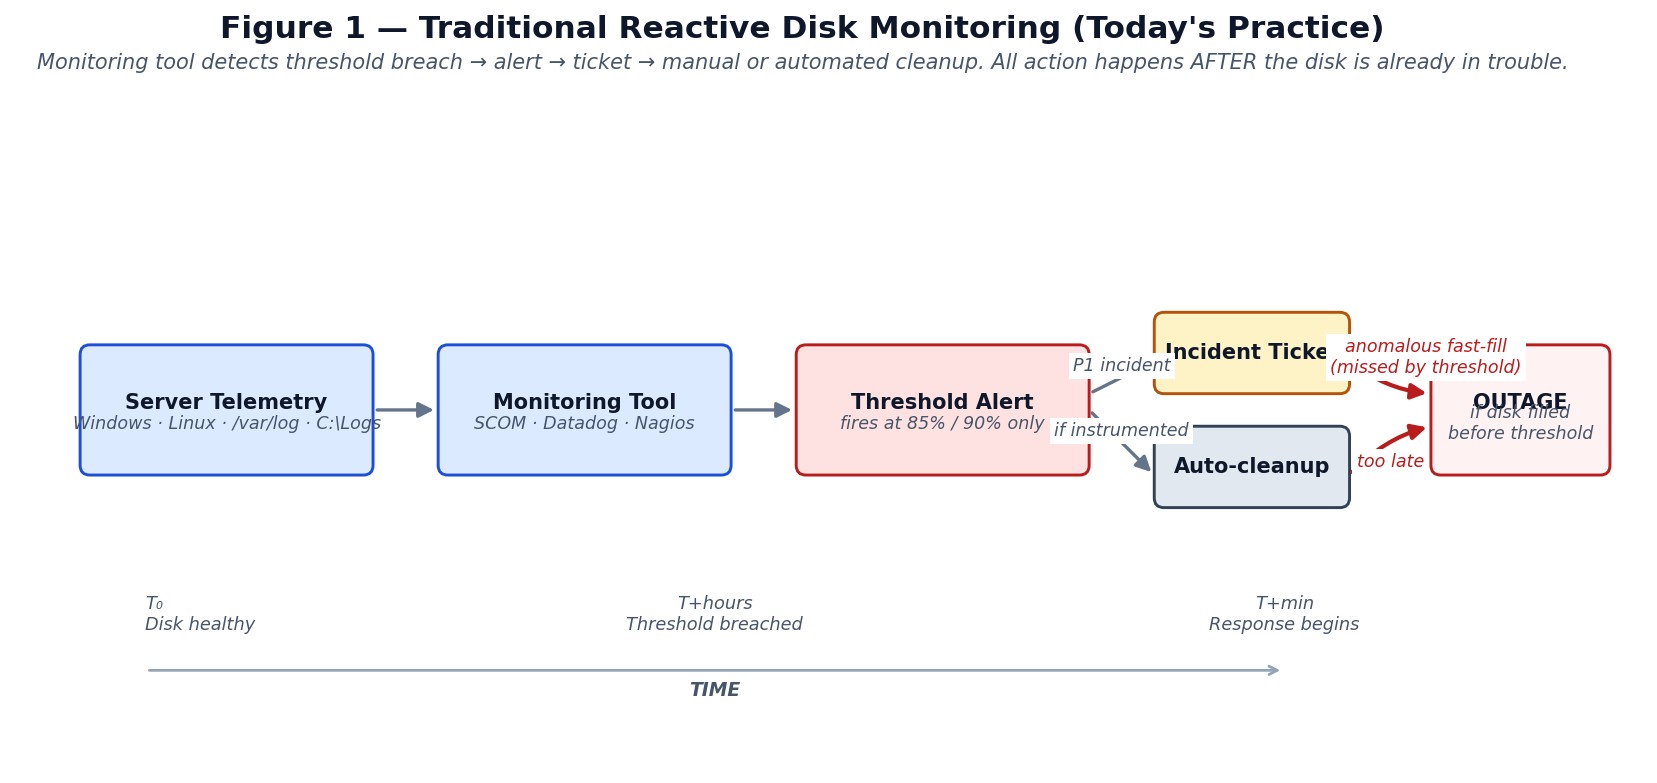
\includegraphics[width=0.9\textwidth]{figure_traditional_flow.png}
\caption{Traditional reactive disk monitoring. All action occurs
\emph{after} a threshold breach, leaving little buffer for response,
particularly under anomalous fast-fill conditions.}
\label{fig:traditional}
\end{figure*}

Server telemetry is collected by a per-host agent (Datadog Agent
\cite{datadog2024disk}, SCOM agent, NRPE for Nagios, etc.) and shipped
to a centralized monitoring platform. The platform evaluates each
host's disk usage against a static threshold; once the threshold is
crossed, an alert dispatches via PagerDuty, Opsgenie, or ServiceNow
\cite{servicenow2024incident}, and an Ops engineer is paged or, in
mature environments, an automated runbook is invoked.

\subsection{Threshold Choices Are Necessarily Conservative}

Any chosen threshold (85--95\% on most production fleets) is a
tradeoff between false-alarm fatigue and response buffer. In practice
most teams settle in the 85--90\% range, which means action begins
only when 85--90\% of the disk is already consumed. For routine
growth this is sufficient; for $10\times$--$100\times$ normal growth,
it is not.

\subsection{Anomalous Fast-Fill: When Monitoring Is Too Late}

The dangerous failure mode is anomalous fast-fill. Common causes
observed in practice:
\begin{itemize}
\item \textbf{DEBUG logging left enabled in production}---a deploy
or a feature flag inadvertently raises the log verbosity.
\item \textbf{Tight retry loops}---a downstream dependency fails, an
upstream service retries aggressively, each failed retry generates a
multi-line error log.
\item \textbf{Misconfigured rotation}---a logrotate or
service-managed rotation policy fails silently.
\item \textbf{Build/batch artifacts}---a CI agent or batch worker
writes intermediate artifacts without cleanup.
\end{itemize}

In each case the volume can saturate within tens of minutes. By the
time a 90\% threshold alert fires, only minutes of buffer remain.

\subsection{Reactive Automation: A Partial Improvement}

Mature teams attach automated cleanup playbooks to disk alerts. This
reduces MTTR for routine cases but does not address anomalous
fast-fill, because (i) the automation is still gated on the
threshold alert, and (ii) the automation runs a static playbook
regardless of why the disk is filling. If growth is anomalous, the
cleanup masks the symptom and the volume re-fills within minutes.

\subsection{The Case for Prediction}

The structural fix is to move action from \emph{after} the threshold
breach to \emph{before}. This requires (i) trajectory awareness
(rate-of-change projection forward) and (ii) pattern awareness
(distinguishing routine accumulation from anomalous growth). Both
are well-studied; the question addressed here is how to combine them
with operational governance into a deployable enterprise system.

%==============================================================
\section{From Reactive to Predictive}
\label{sec:approach}

\subsection{The Disk Guard Approach}

Figure \ref{fig:predictive} shows the predictive flow at single-host
granularity.

\begin{figure*}[t]
\centering
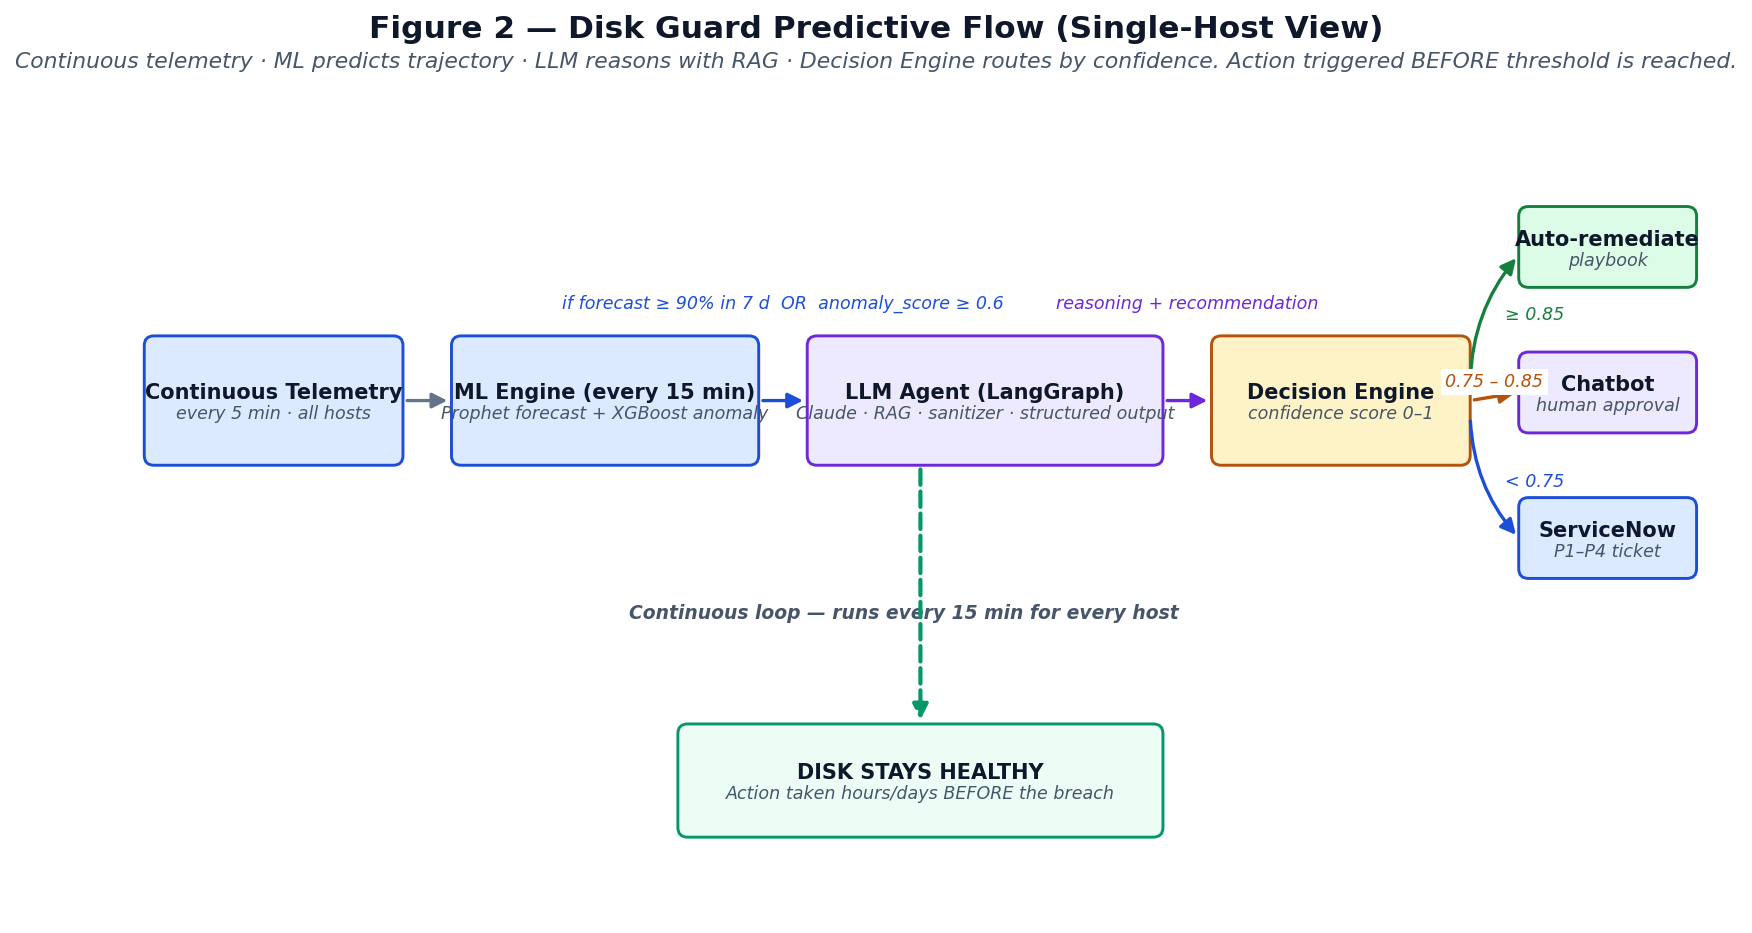
\includegraphics[width=0.95\textwidth]{figure_predictive_flow.png}
\caption{Disk Guard predictive flow. Continuous telemetry feeds a
15-minute ML cycle (Prophet \cite{taylor2018forecasting} + XGBoost
\cite{chen2016xgboost}). Triggered hosts go through an LLM agent
grounded in RAG-retrieved runbooks, with the resulting recommendation
routed by confidence score.}
\label{fig:predictive}
\end{figure*}

Telemetry is collected continuously. Rather than feeding an alert
evaluator, it feeds an ML pipeline that runs every 15 minutes per
host, producing a Prophet forecast at horizons 1, 3, 7, 14 days plus
an XGBoost anomaly score \cite{blazquez2021anomaly}.

A host advances to the next stage if either condition is met:
forecast projects 90\% breach within 7 days, OR anomaly score
$\geq 0.6$. When advanced, the host's full context is presented to
a Claude-powered agent built on a LangGraph
\cite{langchain2024langgraph} state machine. The agent uses
chain-of-thought \cite{wei2022cot} and ReAct \cite{yao2023react}
patterns to produce a structured JSON recommendation.

A Decision Engine combines the agent's self-confidence, the alignment
between agent recommendation and ML signal, the strength of RAG
grounding, and the host's environmental risk profile into a single
0--1 score, mapped to one of three routes: auto-remediate
($\geq 0.85$), chatbot approval ($0.75$--$0.85$), or ServiceNow
ticket only ($<0.75$).

The cycle completes in seconds, intervening while the disk is still
healthy (typically 30--70\% utilization).

\subsection{Side-by-Side Comparison}

Figure \ref{fig:timeline} contrasts the two approaches against a
common incident scenario.

\begin{figure*}[t]
\centering
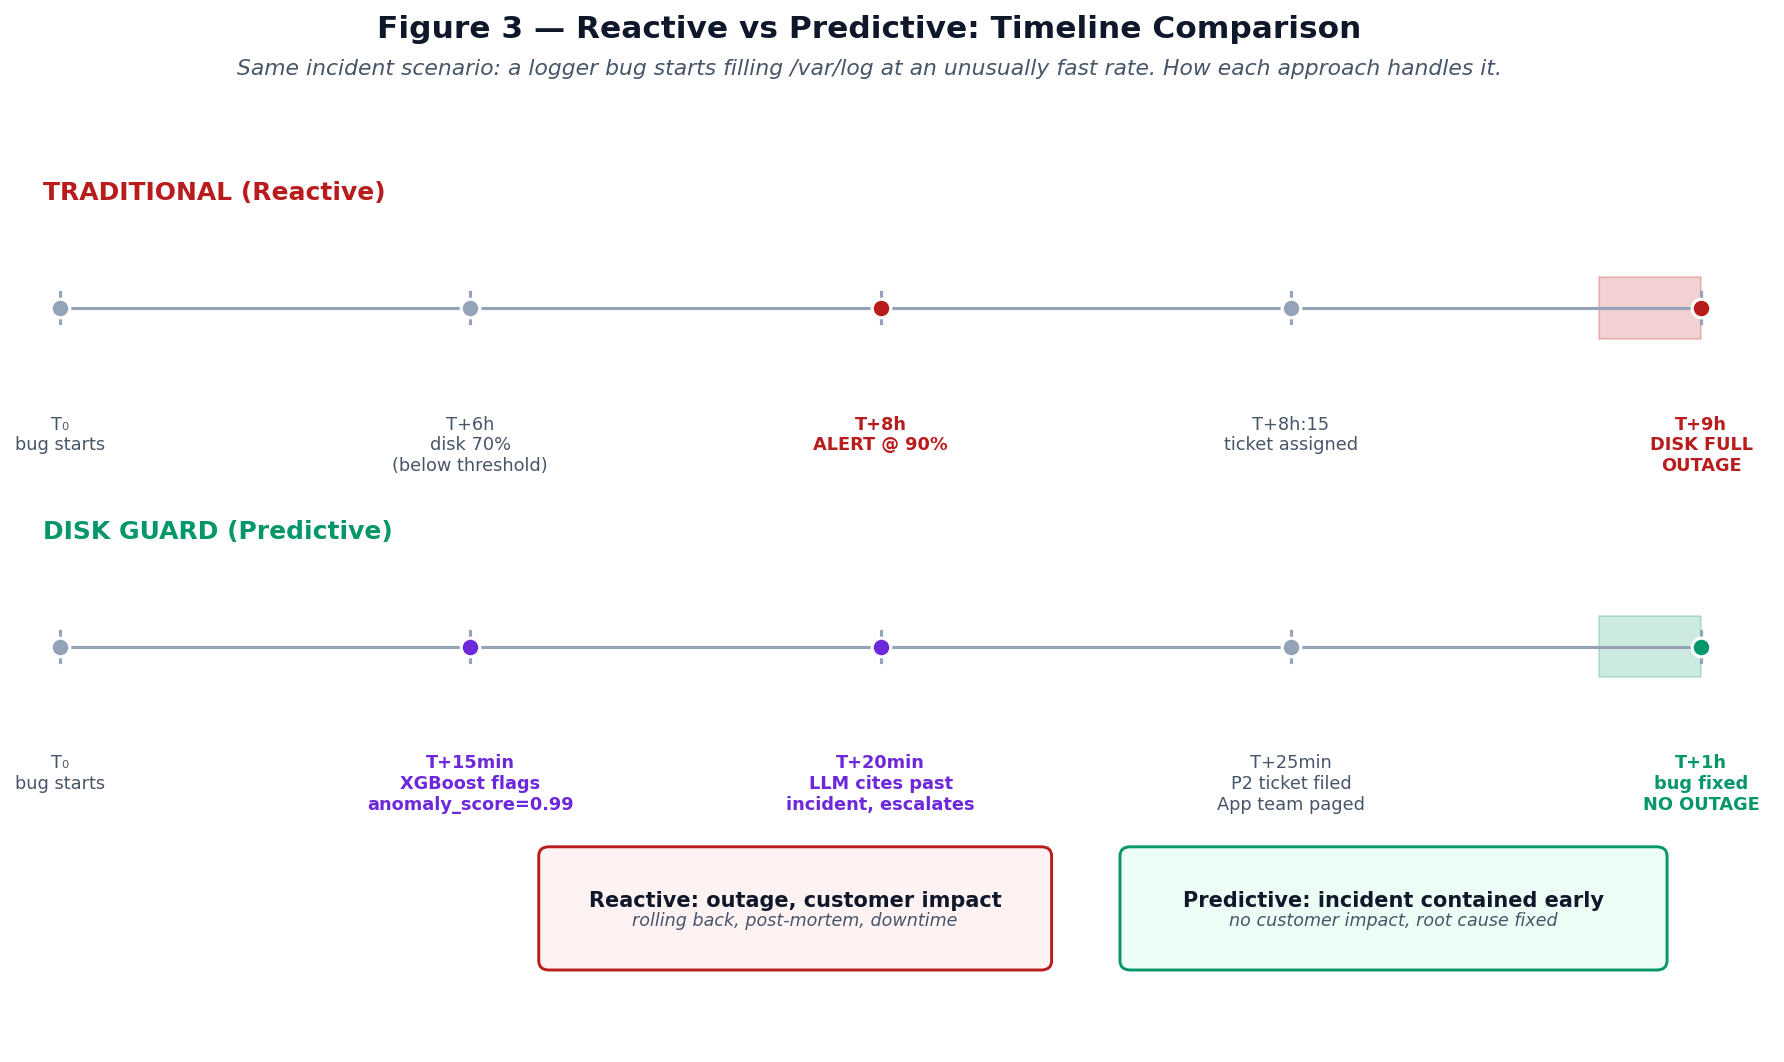
\includegraphics[width=0.95\textwidth]{figure_timeline_comparison.png}
\caption{Reactive vs predictive timelines for the same incident
(deploy-introduced logger bug). Reactive system alerts at T+8h after
threshold breach; outage at T+9h. Predictive system flags anomaly
at T+15min, files P2 ticket at T+25min, root cause fixed at T+1h
with no customer-facing outage.}
\label{fig:timeline}
\end{figure*}

Under the traditional model, the volume crosses 90\% at T+8h,
generating an alert; outage at T+9h. Under Disk Guard, XGBoost
detects the anomalous growth at T+15min, the LLM retrieves
INC-2024-0817 from RAG and recommends escalation, P2 ticket fires
at T+25min, bug rolled back at T+1h. Same telemetry stream, two
fundamentally different outcomes.

%==============================================================
\section{System Architecture}
\label{sec:architecture}

\subsection{Reference Architecture}

The complete architecture appears in Figure \ref{fig:arch},
decomposed into four zones.

\begin{figure*}[t]
\centering
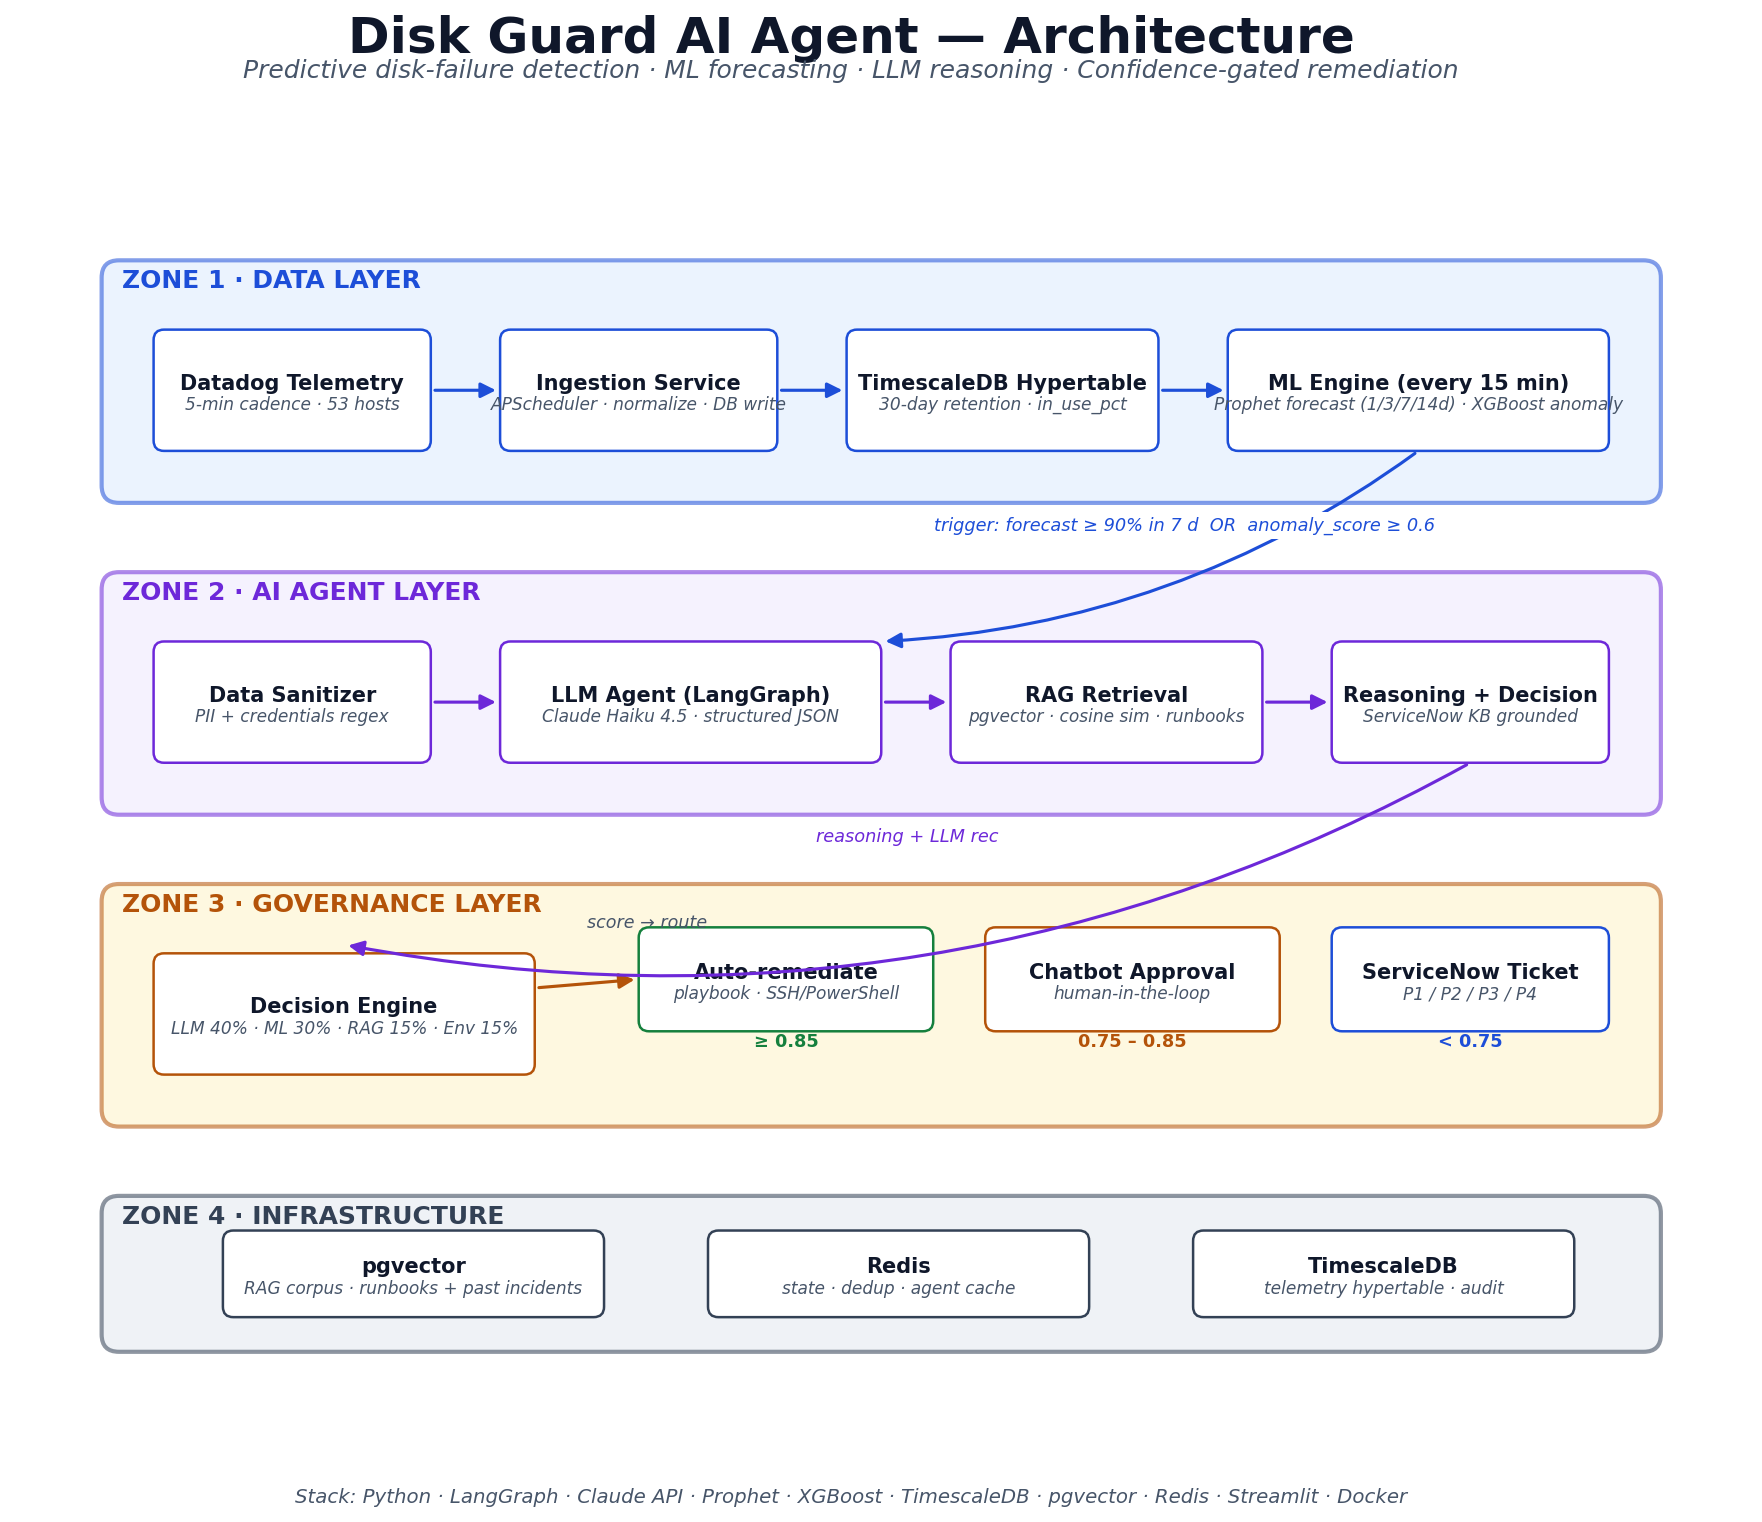
\includegraphics[width=0.95\textwidth]{architecture.png}
\caption{Disk Guard four-zone reference architecture. Each zone has
a well-defined contract with its neighbor: Zone 1 produces triggered
predictions, Zone 2 produces structured LLM recommendations with
self-confidence, Zone 3 routes by confidence score and executes,
Zone 4 provides supporting state and retrieval services.}
\label{fig:arch}
\end{figure*}

The four-zone organization mirrors the canonical layered structure
of modern data-and-ML platforms. Each zone has a well-defined
contract with its neighbors, making components individually
replaceable.

\subsection{Zone 1 --- Data Layer}

Telemetry ingests into a TimescaleDB \cite{timescale2024} hypertable
configured with 30-day retention. Each row records \texttt{(timestamp,
host\_id, device, total\_bytes, used\_bytes, free\_bytes,
in\_use\_pct)}. PostgreSQL \cite{postgresql2024docs} is the
underlying engine. Synthetic telemetry covers 50 simulated hosts;
three real Linux Docker containers provide live-disk validation.

An ingestion service runs every 15 minutes via APScheduler. The ML
Engine runs at the same cadence: per-host Prophet fits + XGBoost
batch scoring + write to \texttt{ml\_predictions}.

\subsection{Zone 2 --- AI Agent Layer}

The agent is a six-node LangGraph state machine
(Figure \ref{fig:agent}).

\begin{figure*}[t]
\centering
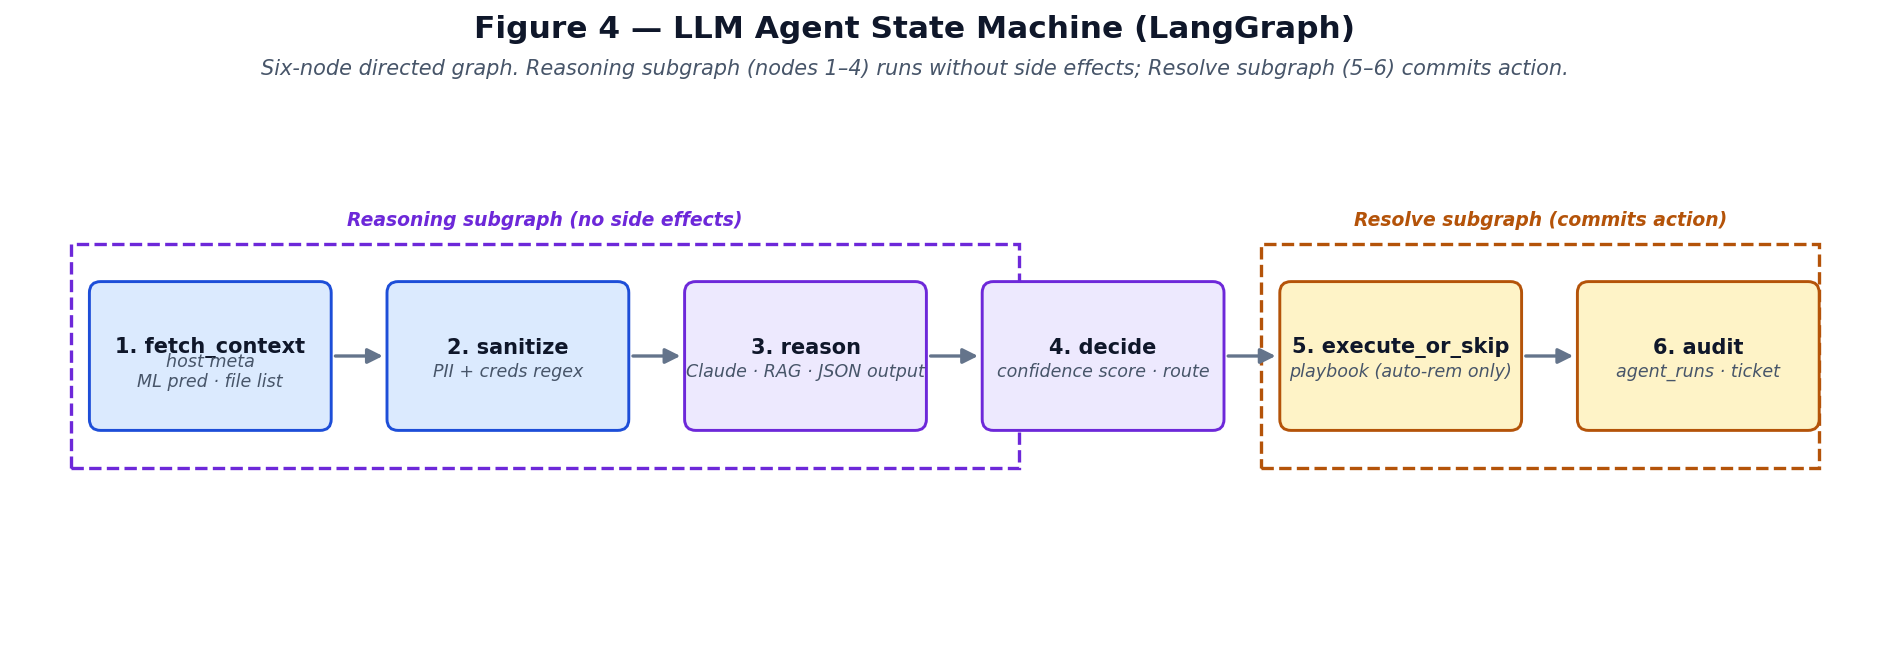
\includegraphics[width=0.95\textwidth]{figure_agent_state_machine.png}
\caption{LangGraph six-node state machine. Reasoning subgraph (1--4)
runs without side effects; Resolve subgraph (5--6) commits action.
The split allows human-in-the-loop interception between reasoning
and execution.}
\label{fig:agent}
\end{figure*}

Nodes 1--4 form the Reasoning subgraph (no side effects). Nodes 5--6
form the Resolve subgraph (commits action). The Reasoning subgraph
gathers context, sanitizes for PII/credentials, invokes the LLM, and
computes the Decision Engine score. The Resolve subgraph executes
the playbook (if route is auto-remediate) and writes the audit row +
ticket.

The reason node submits a structured prompt to Claude Haiku 4.5
\cite{anthropic2024claude3} and parses the JSON response. Embeddings
for RAG use Sentence-BERT \cite{reimers2019sentencebert} indexed
via HNSW \cite{malkov2020hnsw} in pgvector \cite{pgvector2024}.

\subsection{Zone 3 --- Governance Layer}

The Decision Engine is a pure function:
\begin{align*}
\text{score} &= 0.40 \cdot \text{clip}(\text{llm\_self\_confidence}) \\
&+ 0.30 \cdot \text{ml\_alignment}(\text{rec, anomaly, fc}_{7d}) \\
&+ 0.15 \cdot \min(1.0, \text{rag\_doc\_count}/4) \\
&+ \text{env\_boost}[\text{environment}]
\end{align*}

Two hard rules override:
\begin{itemize}
\item LLM recommends \texttt{clean} but \texttt{anomaly\_score}~$>0.6$:
  cap below auto-remediate threshold.
\item LLM recommends \texttt{escalate\_anomaly}: floor at chatbot
  threshold so escalations always reach human review.
\end{itemize}

The Remediation Engine consumes auto-remediate routes via per-role
playbooks (web, app, db). Absolute safety guards: minimum file age
24h, max 80~GB freed per run, max 200 files per run, path whitelist.
The mock ServiceNow client mirrors the Incident table shape.

\subsection{Zone 4 --- Infrastructure Layer}

pgvector \cite{pgvector2024} for the RAG corpus, Redis for state and
deduplication, TimescaleDB \cite{timescale2024} shared with Zone 1.

%==============================================================
\section{Implementation}
\label{sec:impl}

The implementation totals approximately 2{,}500 lines of Python plus
SQL schemas and Docker Compose definitions. Key modules:

\textbf{Synthetic generator.} Stratified across four behavioral
patterns: stable (70\%), declining (15\%), anomalous (10\%),
critical (5\%). Stratified sampling guarantees all patterns appear
at any fleet size.

\textbf{ML Engine.} Prophet \cite{taylor2018forecasting} with linear
growth, daily seasonality, no weekly seasonality, zero uncertainty
samples (point estimates, for performance). XGBoost
\cite{chen2016xgboost} binary classifier on 12 features extracted
from each host's recent series. Trained on a 500-host ephemeral
labeled dataset; 100\% accuracy and 100\% recall on a 25\% holdout.

\textbf{LLM Agent.} Anthropic Claude Haiku 4.5
\cite{anthropic2024claude3} via LangChain Anthropic. Structured JSON
output: \texttt{recommendation} (\texttt{clean} /
\texttt{escalate\_anomaly} / \texttt{no\_action}),
\texttt{self\_confidence} (0--1), \texttt{rationale},
\texttt{key\_evidence}. Per-invocation cost $\sim$USD 0.005.

\textbf{RAG corpus.} Ten seeded documents covering per-role cleanup
runbooks, anomaly-response procedures, a simulated past-incident
record (INC-2024-0817), disk-cleanup safety policy, log retention
requirements, capacity-expansion guidance.

\textbf{Decision Engine.} Pure Python function with exhaustive unit
tests; weights and thresholds in configuration.

\textbf{Remediation Engine.} Per-role playbooks as ordered glob +
min-age rules; executor walks each rule's matches via \texttt{find}
inside the container, applies safety guards, and deletes via
\texttt{rm}.

\textbf{ServiceNow integration.} Mock client mirrors the Incident
table shape; production deployment swaps for the real
\texttt{api/now/table/incident} REST client.

%==============================================================
\section{Operational Workflow}
\label{sec:flow}

The Streamlit demonstration UI structures interaction around four
numbered stages:

\textbf{Stage 1 --- Monitor.} Host's disk-usage trajectory over
24h/3d/7d. Fill Disk simulator writes sparse files to demonstrate
fill behavior.

\textbf{Stage 2 --- Predict.} Click runs Prophet + XGBoost; metrics
displayed (anomaly, forecast 1d/7d, hours-to-90\%, triggered).
Freshness indicator shows prediction timestamp.

\textbf{Stage 3 --- Reasoning.} Click runs LangGraph reasoning
subgraph; LLM rationale, key evidence, and Decision Engine score
shown. \emph{No side effects}: no audit row, no ticket, no
remediation. Operator reviews before committing.

\textbf{Stage 4 --- Resolve.} Click runs Resolve subgraph: executes
playbook (if auto-remediate + LLM recommended clean), files ticket
(if escalate or ticket-only), writes audit row.

\subsection{Worked Example: Anomalous-Growth Refusal}

Consider the scenario in Figure \ref{fig:timeline}. At T+15min after
a logger bug begins:
\begin{itemize}
\item \texttt{anomaly\_score} = 0.997
\item \texttt{forecast\_7d\_pct} = 100.0
\item \texttt{hours\_to\_90pct} = 24.1
\end{itemize}

The LLM retrieves INC-2024-0817 from RAG and returns:
\begin{quote}\itshape
``Anomaly score of 0.997 combined with a single massive file
(\texttt{app-debug.log}, 64 GB, age 0 days) exhibiting explosive
growth is a textbook upstream incident signature. INC-2024-0817
demonstrates that cleanup of anomalous growth merely delays the
inevitable disk fill; the correct response is to identify the
upstream cause and remediate it.''
\end{quote}

The Decision Engine score:
\begin{align*}
\text{score} &= 0.40(0.98) + 0.30(0.997) + 0.15(1.0) + 0.05 \\
&= 0.391 + 0.299 + 0.150 + 0.050 = 0.890
\end{align*}

Route: auto-remediate. But the execute node observes the LLM did not
recommend \texttt{clean} and skips the playbook. The audit node sets
verdict to \texttt{escalated\_anomaly} and files P2 ticket
INC-2026-05-0001 (assignment group \texttt{App-Support-app}). No
files are deleted.

%==============================================================
\section{Validation}
\label{sec:validation}

\textbf{Test fleet.} 53 hosts: 50 simulated (stratified across four
patterns) plus three real Linux containers (web, app, db). Synthetic
telemetry: $\sim$100{,}800 rows in \texttt{disk\_telemetry} for the
seven-day backfill at five-minute cadence.

\textbf{Scenario A --- Predictive cleanup.} Forecast $\sim$100\%,
anomaly $\sim$0.003. LLM recommends \texttt{clean}. Decision Engine
$\sim$0.87 $\Rightarrow$ auto-remediate. Four rotated archives
deleted, $\sim$16~GB freed. Verdict: \texttt{cleaned}.

\textbf{Scenario B --- Anomaly refusal.} Forecast $\sim$100\%,
anomaly $\sim$0.997. LLM recommends \texttt{escalate\_anomaly},
citing INC-2024-0817. Decision Engine $\sim$0.89 $\Rightarrow$
auto-remediate route, but execute correctly skips. P2 ticket filed.
No files deleted. Verdict: \texttt{escalated\_anomaly}.

\textbf{Performance.}
\begin{itemize}
\item Full ML cycle (53 hosts): $\sim$8 seconds.
\item Single-host on-demand prediction: $\sim$3 seconds.
\item End-to-end agent invocation: 8--15 seconds (Claude API-bound).
\item XGBoost holdout accuracy: 100\% on 125-host stratified test
  split (synthetic data; production accuracy bounded by quality of
  historical incident labeling).
\end{itemize}

%==============================================================
\section{Discussion}
\label{sec:discussion}

\subsection{Comparison with Related Work}

Predictive disk monitoring is not new---capacity-planning tools have
offered linear extrapolation for decades, and the broader literature
on online failure prediction is well-developed
\cite{salfner2010survey,lin2018predicting}. What is novel here is
the \emph{integration}: modern time-series forecasting
\cite{taylor2018forecasting}, a dedicated gradient-boosted anomaly
classifier \cite{chen2016xgboost}, retrieval-augmented LLM reasoning
\cite{lewis2020rag,brown2020gpt3}, and an explicit governance layer.
Each component has been deployed in isolation in AIOps systems
\cite{notaro2021aiops}; the joint deployment, structured around the
four-zone architecture, is the contribution.

\subsection{Limitations}

\begin{itemize}
\item Synthetic telemetry only (no real Datadog ingestion in POC).
\item Mock ServiceNow integration (real REST client deferred).
\item Synthetic RAG corpus (10 documents).
\item Single-domain scope (disk only).
\item POC scale (50 simulated + 3 real hosts) below the architecture's
  3{,}000-host design target.
\item Hard dependency on Anthropic Claude API; degraded mode
  defaults to ticket-only if API unavailable.
\end{itemize}

\subsection{Production Considerations}

Credential management (vault-sourced rather than env vars), per-host
trust configuration for auto-remediate eligibility, audit retention
matching organizational compliance requirements, and scheduled model
retraining are all required before production deployment.

\subsection{Generalization}

The four-zone reference architecture generalizes to other AIOps
problems: service-uptime prediction, backup-job-failure prediction,
storage capacity planning, network bandwidth saturation. Disk Guard
is best understood as the first instance of a reusable pattern.

%==============================================================
\section{Future Work}
\label{sec:future}

\begin{enumerate}
\item Real Datadog ingestion and validation against production
  telemetry corpora.
\item Per-host learned baselines (each host learns its own expected
  growth rate).
\item Cross-host correlation for fleet-wide signals from common
  upstream causes.
\item Local-model fallback for the reasoning step during API outages.
\item A reusable per-tower agent library (services, backups, storage,
  network) sharing the Disk Guard architecture.
\item Active learning from operator approve/deny signals in the
  chatbot path.
\end{enumerate}

%==============================================================
\section{Conclusion}
\label{sec:conclusion}

Disk-fill is a well-understood failure class with well-understood
operational cost. The dominant mitigation today---threshold-based
monitoring with reactive cleanup---handles routine cases reasonably
well and fails badly at exactly the moments when getting it right
matters most: the anomalous fast-fill cases driven by deploy
regressions and runaway processes. The structural fix is simple to
state: stop waiting for the threshold breach. Watch the trajectory
instead. Act before the disk is in trouble, not after.

That is what I set out to build with Disk Guard AI Agent, and that
is what this paper has described. The system continuously forecasts
disk-fill trajectories using Prophet \cite{taylor2018forecasting},
classifies anomalous growth patterns with XGBoost
\cite{chen2016xgboost}, and asks a Claude-powered LangGraph agent
\cite{anthropic2024claude3,langchain2024langgraph}---grounded in
retrieved runbook and past-incident content \cite{lewis2020rag}---to
reason about what to do. The resulting recommendation is then scored
and routed by an explicit governance layer.

The system works. On the 53-host POC fleet it produces correct,
explainable decisions in seconds rather than minutes. It tells
routine cleanup opportunities apart from anomalous-growth incidents.
When the LLM recommends escalation rather than cleanup, the executor
correctly refuses to delete files and a P2 ticket is filed instead.

The contribution is not a new algorithm. It is a working composition
pattern: how to combine forecasting, anomaly detection, LLM
reasoning, retrieval, and governance into a system that can be
deployed in real IT-operations environments without giving up
either safety or transparency. The same pattern applies directly to
service uptime, backup verification, storage capacity, and network
bandwidth.

The complete source code, architecture diagrams, demonstration
scripts, and reproduction instructions are at the repository cited
above. I welcome feedback, contributions, and replication on real
production telemetry.

%==============================================================
\section*{Acknowledgments}

The author thanks Tata Consultancy Services for sponsoring the
research program under which this work was developed, and the broader
TCS Infrastructure Operations community for grounding insight on
real-world disk-incident patterns. The author is also grateful to the
open-source maintainers of Prophet, XGBoost, LangGraph, LangChain,
sentence-transformers, pgvector, TimescaleDB, Redis, Streamlit, and
Docker, whose work this implementation rests upon, and to Anthropic
for the Claude API and SDK.

\textbf{Disclosure of AI assistance.} Portions of this manuscript
were drafted with assistance from Anthropic's Claude large language
model (model: \texttt{claude-haiku-4-5}; integration: Anthropic
Python SDK), under the direct guidance, factual review, and final
editorial approval of the author. All technical claims, architectural
decisions, implementation details, market estimates, and validation
results reflect the author's own work. The author is solely
responsible for the content, accuracy, and conclusions of this paper,
in accordance with the IEEE Author Center's policy on the use of
generative artificial intelligence in scientific writing.

%==============================================================
\bibliographystyle{IEEEtran}
\bibliography{references}

\end{document}
